\section{Results}\label{sec:results}

\subsection{Retrieval}\label{sec:res-retrieval}
Table~\ref{tab:main} gives Hit@5 on the generation queries; Table~\ref{tab:ci} gives the intervals. On NQ, the dense encoders spread widely. MiniLM-L6 reached \ev{HIT.nq.R1} and e5-base-v2 \ev{HIT.nq.R5}; bge-large (\ev{HIT.nq.R4}) came second. Qwen3-Embedding-0.6B (\ev{HIT.nq.R6}) placed between bge-small and bge-base. BM25 reached \ev{HIT.nq.R0}. On HotpotQA, Hit@5 nearly saturated: all dense encoders except MiniLM-L6 scored between \ev{HIT.hp.R6} and \ev{HIT.hp.R4}, against \ev{HIT.hp.R1} for MiniLM-L6 and \ev{HIT.hp.R0} for BM25. The stricter Both@5 separated them more clearly: bge-large found both supporting passages for \ev{BOTH.hp.R4} of the questions, e5-base-v2 for \ev{BOTH.hp.R5}, Qwen3-Embedding-0.6B for \ev{BOTH.hp.R6} and MiniLM-L6 for \ev{BOTH.hp.R1}.

\subsection{Answers and transfer (RQ1)}\label{sec:res-transfer}
Table~\ref{tab:main} gives EM for every cell with its two bounds, and Fig.~\ref{fig:hitem} plots EM against Hit@5. Retrieval closed only part of the gap between the closed-book and gold-passage conditions. With Qwen on NQ, closed-book EM was \ev{EM.qnq.CB}, gold passages gave \ev{EM.qnq.GOLD}, and the best retriever, e5-base-v2, gave \ev{EM.qnq.R5}. With Llama on NQ the best retriever was bge-base (\ev{EM.lnq.R3}) against a gold bound of \ev{EM.lnq.GOLD}. On HotpotQA, bge-large gave the highest EM for both readers (\ev{EM.qhp.R4} and \ev{EM.lhp.R4}), against gold bounds of \ev{EM.qhp.GOLD} and \ev{EM.lhp.GOLD}.

\begin{figure}[t]
\centering
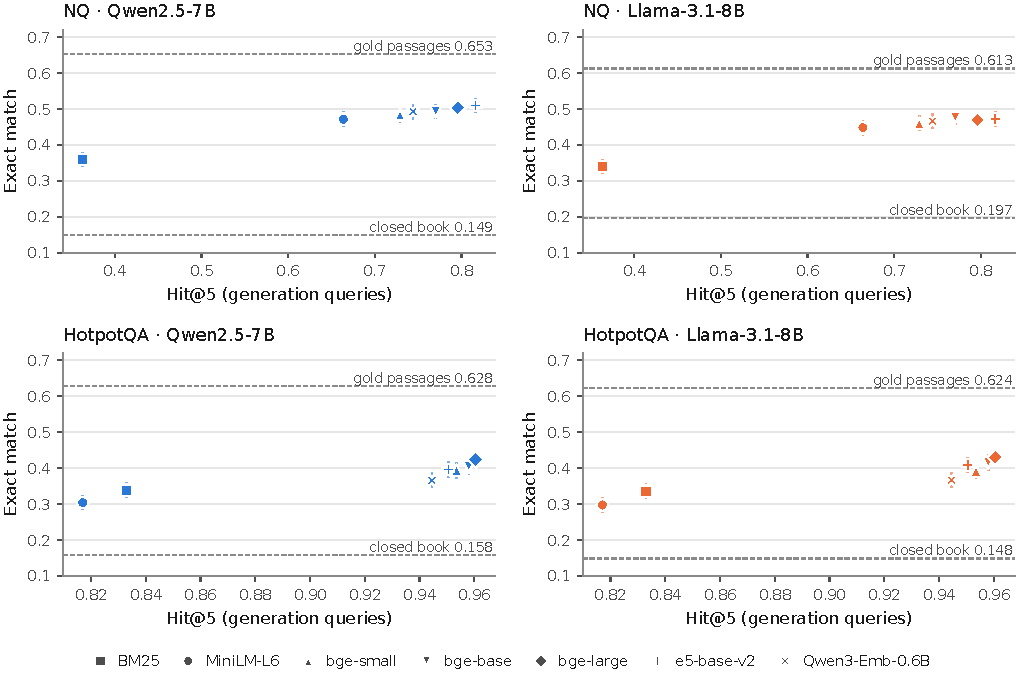
\includegraphics[width=\linewidth]{figs/fig2_hit_vs_em.pdf}
\caption{Exact match against Hit@5 for each retriever in the four reader--dataset cells. Vertical bars are 95\% bootstrap intervals for EM. Dashed lines mark the closed-book and gold-passage conditions. Note the different Hit@5 ranges of the two datasets.}
\label{fig:hitem}
\end{figure}

Table~\ref{tab:transfer} and Fig.~\ref{fig:transfer} give the transfer ratios. On NQ, the dense encoders had ratios between \ev{T.lnq.R4} (bge-large and e5-base-v2 with Llama) and \ev{T.lnq.R3} (bge-base with Llama). With Qwen, e5-base-v2 gained \ev{DH.qnq.R5} in Hit@5 over MiniLM-L6 but only \ev{DE.qnq.R5} in EM, a ratio of \ev{T.qnq.R5} \ev{T.qnq.R5.ci}. The intervals for bge-small included zero in both NQ cells (Qwen \ev{T.qnq.R2.ci}, Llama \ev{T.lnq.R2.ci}), so its NQ ratio is uncertain in sign. No upper bound on NQ exceeded \ev{T.qnq.R6.hi}. BM25 retrieved worse than MiniLM-L6 on NQ, so its ratio (\ev{T.qnq.R0} with Qwen) describes how much of the retrieval loss reached the answer.

On HotpotQA the ratios were larger for every encoder and reader. They ranged from \ev{T.qhp.R6} (Qwen3-Embedding-0.6B with Qwen) to \ev{T.lhp.R4} (bge-large with Llama). With Qwen, every upper bound stayed below 1, the largest being \ev{T.qhp.R4.hi3} for bge-large. With Llama, the bounds were \ev{T.lhp.R3.hi3} for bge-base, \ev{T.lhp.R5.hi3} for e5-base-v2 and \ev{T.lhp.R4.hi3} for bge-large; three of five bounds reached or exceeded 1. Prediction P1 therefore held in the two new NQ and Qwen--HotpotQA cells and failed in the Llama--HotpotQA cell (Table~\ref{tab:predictions}). The BM25 ratio was not estimable on HotpotQA, because BM25 and MiniLM-L6 differed by only \ev{DH.qhp.R0} in Hit@5.

\begin{figure}[t]
\centering
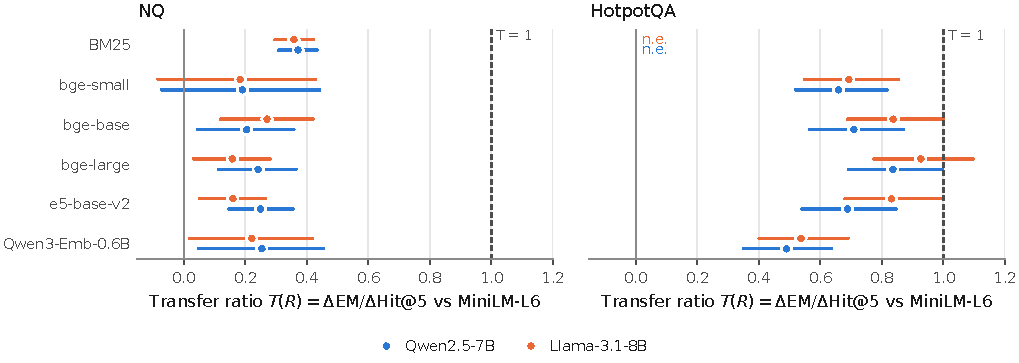
\includegraphics[width=\linewidth]{figs/fig1_transfer_ratios.pdf}
\caption{Transfer ratio $T(R)=\Delta\mathrm{EM}/\Delta\mathrm{Hit@5}$ against MiniLM-L6 with 95\% bootstrap intervals. The dashed line marks $T=1$. n.e.: not estimable under the reporting rule.}
\label{fig:transfer}
\end{figure}

\begin{table*}[t]
\centering
\small
\caption{Retrieval (Hit@5) and answer quality (exact match) for each reader and dataset. Hit@5 is computed on the generation queries; 95\% bootstrap intervals are in Table~\ref{tab:ci}.}
\label{tab:main}
\begin{tabular}{lrrrrrrrr}
\toprule
 & \multicolumn{4}{c}{NQ (2,255 queries)} & \multicolumn{4}{c}{HotpotQA (2,000 queries)} \\ \cmidrule(lr){2-5}\cmidrule(lr){6-9} & \multicolumn{2}{c}{Qwen} & \multicolumn{2}{c}{Llama} & \multicolumn{2}{c}{Qwen} & \multicolumn{2}{c}{Llama} \\ \cmidrule(lr){2-3}\cmidrule(lr){4-5}\cmidrule(lr){6-7}\cmidrule(lr){8-9}
Retriever & Hit@5 & EM & Hit@5 & EM & Hit@5 & EM & Hit@5 & EM \\
\midrule
BM25 & 0.363 & 0.360 & 0.363 & 0.340 & 0.833 & 0.339 & 0.833 & 0.336 \\
MiniLM-L6 & 0.664 & 0.471 & 0.664 & 0.448 & 0.817 & 0.304 & 0.817 & 0.297 \\
bge-small & 0.729 & 0.484 & 0.729 & 0.460 & 0.954 & 0.394 & 0.954 & 0.392 \\
bge-base & 0.770 & 0.493 & 0.770 & 0.477 & 0.958 & 0.404 & 0.958 & 0.415 \\
bge-large & 0.796 & 0.503 & 0.796 & 0.469 & 0.961 & 0.424 & 0.961 & 0.430 \\
e5-base-v2 & 0.816 & 0.510 & 0.816 & 0.472 & 0.951 & 0.396 & 0.951 & 0.408 \\
Qwen3-Emb-0.6B & 0.744 & 0.492 & 0.744 & 0.466 & 0.945 & 0.366 & 0.945 & 0.366 \\
Closed book & -- & 0.149 & -- & 0.197 & -- & 0.158 & -- & 0.148 \\
Gold passages & -- & 0.653 & -- & 0.613 & -- & 0.628 & -- & 0.624 \\
\bottomrule
\end{tabular}
\end{table*}

\begin{table*}[t]
\centering
\small
\caption{Transfer ratio $T(R)=\Delta\mathrm{EM}/\Delta\mathrm{Hit@5}$ relative to MiniLM-L6, with 95\% bootstrap intervals.}
\label{tab:transfer}
\begin{tabular}{lcccc}
\toprule
Retriever & NQ Qwen & NQ Llama & HotpotQA Qwen & HotpotQA Llama \\
\midrule
BM25 & 0.37 [0.31, 0.43] & 0.36 [0.30, 0.42] & n.e. & n.e. \\
bge-small & 0.19 [$-$0.07, 0.44] & 0.18 [$-$0.08, 0.43] & 0.66 [0.52, 0.82] & 0.69 [0.55, 0.85] \\
bge-base & 0.20 [0.04, 0.36] & 0.27 [0.12, 0.42] & 0.71 [0.57, 0.87] & 0.84 [0.69, 1.00] \\
bge-large & 0.24 [0.11, 0.36] & 0.16 [0.03, 0.28] & 0.84 [0.69, 1.00] & 0.93 [0.78, 1.10] \\
e5-base-v2 & 0.25 [0.15, 0.36] & 0.16 [0.05, 0.26] & 0.69 [0.54, 0.85] & 0.83 [0.68, 1.00] \\
Qwen3-Emb-0.6B & 0.25 [0.05, 0.45] & 0.22 [0.02, 0.42] & 0.49 [0.35, 0.64] & 0.54 [0.40, 0.69] \\
\bottomrule
\end{tabular}
\par\smallskip\parbox{\linewidth}{\footnotesize n.e.: not estimable under the pre-registered rule ($|\Delta\mathrm{Hit@5}|\le 2$ points or not significant after Holm). BM25 on NQ retrieves worse than MiniLM-L6, so its ratio describes a loss.}
\end{table*}


The lenient answer metrics moved the ratios up but did not change the pattern (Table~\ref{tab:transferalt}). With token F1, the NQ ratios of the dense encoders stayed between \ev{TF.lnq.R2} and \ev{TF.lnq.R3}. On HotpotQA with Llama, the F1 ratio of bge-large was \ev{TF.lhp.R4} \ev{TF.lhp.R4.ci}, so under F1 a full transfer cannot be ruled out for that encoder.

\subsection{Where the transfer comes from}\label{sec:res-decomp}
The decomposition in Eq.~\ref{eq:decomp} separates two effects (Table~\ref{tab:decomp}). One term, the hit--miss gap of MiniLM-L6, was similar in all cells: \ev{DB.qnq} and \ev{DB.lnq} on NQ, \ev{DB.qhp} and \ev{DB.lhp} on HotpotQA. The other term differed in sign between the datasets.

On NQ it was negative for every dense encoder (from \ev{DR.lnq.R4} to \ev{DR.lnq.R3} with Llama; from \ev{DR.qnq.R2} to \ev{DR.qnq.R6} with Qwen). Better encoders found gold passages for more questions, but EM given a hit fell slightly (Qwen: \ev{PH.qnq.R1} for MiniLM-L6, \ev{PH.qnq.R5} for e5-base-v2). EM given a miss stayed near \ev{PM.qnq.R5}, well above closed-book EM (\ev{EM.qnq.CB}). A ``miss'' under the sparse NQ labels thus often still produced a correct answer.

On HotpotQA the second term was positive and large, from \ev{DR.qhp.R6} (Qwen3-Embedding-0.6B with Qwen) to \ev{DR.lhp.R4} (bge-large with Llama). It made up \ev{DS.hp.min} to \ev{DS.hp.max} of the ratio. EM given a hit rose with the encoder (Qwen: \ev{PH.qhp.R1} for MiniLM-L6, \ev{PH.qhp.R4} for bge-large), while EM given a miss was lower for the stronger encoders (Qwen: \ev{PM.qhp.R1} for MiniLM-L6, \ev{PM.qhp.R5} to \ev{PM.qhp.R6} for the others). The rise matches the Both@5 results: better encoders more often retrieved the second supporting passage, which Hit@5 does not count. In a post hoc check, the EM ranking of the seven retrievers equalled their Both@5 ranking in both HotpotQA cells (Spearman $\rho$ = \ev{RHOB.qhp} and \ev{RHOB.lhp}); against Hit@5 it was \ev{RHO.qhp} and \ev{RHO.lhp}. Bridge questions drove this. With Qwen, bridge EM rose from \ev{BT.qhp.bridge.R1} (MiniLM-L6) to \ev{BT.qhp.bridge.R4} (bge-large), while comparison EM moved from \ev{BT.qhp.comparison.R1} to \ev{BT.qhp.comparison.R4}, close to its gold bound of \ev{BT.qhp.comparison.GOLD}.

\subsection{Encoder comparisons (RQ2)}\label{sec:res-encoders}
Prediction P2 held on NQ and failed on HotpotQA (Table~\ref{tab:predictions}). On NQ, neither bge-large nor Qwen3-Embedding-0.6B differed detectably from e5-base-v2 in EM with either reader. On HotpotQA, bge-large gave higher EM than e5-base-v2 with both readers (\ev{P2.qhp.R4}, Holm-adjusted $p$ = \ev{P2.qhp.R4.p}; \ev{P2.lhp.R4}, $p$ = \ev{P2.lhp.R4.p}), in line with its higher Both@5. Qwen3-Embedding-0.6B gave lower EM than e5-base-v2 on HotpotQA (\ev{P2.qhp.R6}, $p$ = \ev{P2.qhp.R6.p}; \ev{P2.lhp.R6}, $p$ = \ev{P2.lhp.R6.p}). The pooled model over all four cells (Table~\ref{tab:gee}; \ev{GEE.rows} answers in \ev{GEE.clusters} query clusters) gave the same picture: odds ratio \ev{GEE.or.R4} \ev{GEE.ci.R4} for bge-large and \ev{GEE.or.R6} \ev{GEE.ci.R6} for Qwen3-Embedding-0.6B, each against e5-base-v2. The bge-large advantage was small and its interval nearly touched 1. The pooled model mixes the two study phases and is secondary.

\begin{table}[t]
\centering
\small
\caption{Pooled GEE logistic model of EM over the four reader--dataset cells.}
\label{tab:gee}
\begin{tabular}{lcc}
\toprule
Contrast & Odds ratio [95\% CI] & $p$ \\
\midrule
bge-large vs e5-base-v2 & 1.038 [1.001, 1.076] & 0.043 \\
Qwen3-Emb-0.6B vs e5-base-v2 & 0.909 [0.875, 0.943] & $<$0.001 \\
\bottomrule
\end{tabular}
\par\smallskip\parbox{\linewidth}{\footnotesize EM $\sim$ retriever + dataset + reader; exchangeable working correlation (0.60) within query; 59,570 answers in 4,255 query clusters; empirical (sandwich) standard errors.}
\end{table}


\subsection{Context choices (RQ3)}\label{sec:res-context}
\paragraph{Number of passages}
Table~\ref{tab:topk} and Fig.~\ref{fig:topk} show EM for $k\in\{1,3,5,10\}$ with Qwen on NQ. One passage gave lower EM than five for every retriever (P4 held; differences from \ev{K1.R0} for BM25 to \ev{K1.R5} for e5-base-v2, all Holm-adjusted $p<0.001$). From five to ten passages, EM rose for six retrievers and stayed flat for e5-base-v2 (\ev{TK.R5.k5} and \ev{TK.R5.k10}). The gap between retrievers shrank with $k$: at $k=10$ all dense encoders gave EM between \ev{TK.R1.k10} and \ev{TK.R4.k10}.

\begin{figure}[t]
\centering
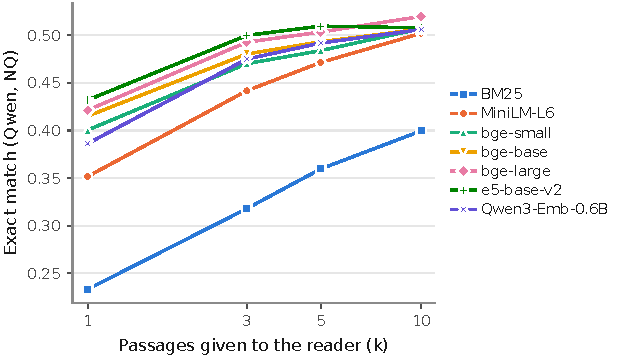
\includegraphics[width=0.85\linewidth]{figs/fig3_topk.pdf}
\caption{Exact match by number of passages $k$, Qwen reader on NQ (2,255 queries).}
\label{fig:topk}
\end{figure}

\paragraph{Passage composition and position}
Table~\ref{tab:mechanism} and Fig.~\ref{fig:mechanism} give the controlled context test on 500 NQ questions. With the gold passage at position 1, four top-ranked non-gold BM25 passages gave EM \ev{MC.M1}, and four random passages gave \ev{MC.MR}: a drop of \ev{P5.abs} (exact McNemar $p$ = \ev{P5.p}; P5 held). Random passages were harmless: gold at position 1 plus four random passages did not differ detectably from the gold passage alone (\ev{MC.MG}; $p$ = \ev{MG.p}). The position of the gold passage among the hard negatives showed no detectable effect (EM \ev{MC.M1}, \ev{MC.M3} and \ev{MC.M5} at positions 1, 3 and 5; all Holm-adjusted $p\ge$ \ev{P6.M1M3.p}; P6 failed).

\begin{figure}[t]
\centering
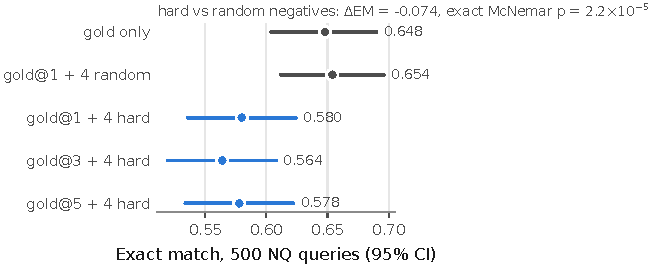
\includegraphics[width=0.75\linewidth]{figs/fig4_mechanism.pdf}
\caption{Exact match for five controlled contexts of five passages (Qwen reader, 500 NQ generation queries) with 95\% bootstrap intervals.}
\label{fig:mechanism}
\end{figure}

\begin{table}[t]
\centering
\small
\caption{Exact match by number of passages $k$ (Qwen reader, NQ, 2,255 queries).}
\label{tab:topk}
\begin{tabular}{lrrrrrr}
\toprule
Retriever & $k{=}1$ & $k{=}3$ & $k{=}5$ & $k{=}10$ & $\Delta_{1-5}$ & $p_\text{Holm}$ \\
\midrule
BM25 & 0.233 & 0.318 & 0.360 & 0.400 & $-$0.126 & $<$0.001 \\
MiniLM-L6 & 0.352 & 0.442 & 0.471 & 0.502 & $-$0.120 & $<$0.001 \\
bge-small & 0.400 & 0.470 & 0.484 & 0.507 & $-$0.083 & $<$0.001 \\
bge-base & 0.415 & 0.480 & 0.493 & 0.506 & $-$0.078 & $<$0.001 \\
bge-large & 0.421 & 0.493 & 0.503 & 0.520 & $-$0.082 & $<$0.001 \\
e5-base-v2 & 0.432 & 0.500 & 0.510 & 0.508 & $-$0.078 & $<$0.001 \\
Qwen3-Emb-0.6B & 0.386 & 0.475 & 0.492 & 0.506 & $-$0.106 & $<$0.001 \\
\bottomrule
\end{tabular}
\par\smallskip\parbox{\linewidth}{\footnotesize Exact McNemar test of $k{=}1$ vs $k{=}5$, Holm over seven retrievers.}
\end{table}

\begin{table}[t]
\centering
\small
\caption{Distraction and position tests (Qwen reader, 500 NQ generation queries).}
\label{tab:mechanism}
\begin{tabular}{lccc}
\toprule
Context (5 passages) & EM [95\% CI] & F1 & AC \\
\midrule
Gold only & 0.648 [0.604, 0.690] & 0.772 & 0.770 \\
Gold@1 + 4 random & 0.654 [0.612, 0.696] & 0.777 & 0.764 \\
Gold@1 + 4 hard & 0.580 [0.536, 0.624] & 0.696 & 0.686 \\
Gold@3 + 4 hard & 0.564 [0.520, 0.608] & 0.684 & 0.672 \\
Gold@5 + 4 hard & 0.578 [0.534, 0.622] & 0.698 & 0.682 \\
\bottomrule
\end{tabular}
\par\smallskip\parbox{\linewidth}{\footnotesize Hard vs random negatives: $\Delta$EM = $-$0.074, exact McNemar $p$ = $2.2\times10^{-{}5}$. Position: no pair differs after Holm.}
\end{table}


\paragraph{Reranking}
The cross-encoder helped BM25 and hurt e5-base-v2 (Table~\ref{tab:reranker}). On the NQ generation queries, reranking the BM25 top 50 raised Hit@5 by \ev{RR.X0_vs_R0.hit} and EM by \ev{RR.X0_vs_R0.em} (both $p<0.001$). Reranking the e5-base-v2 top 50 lowered Hit@5 by \ev{RR.X5_vs_R5.hit} ($p$ = \ev{RR.X5_vs_R5.hit.p}); for EM the change was \ev{RR.X5_vs_R5.em} ($p$ = \ev{RR.X5_vs_R5.em.p}), and no difference was detected. Reranking cost a median of \ev{RR.lat.R0} to \ev{RR.lat.R5}~ms per query on a T4. These results come from one reranker at one depth.

\begin{table}[t]
\centering
\small
\caption{Cross-encoder reranking (bge-reranker-base, top 50) on NQ.}
\label{tab:reranker}
\begin{tabular}{lcccc}
\toprule
System & Hit@5 & nDCG@10 & EM & ms/query \\
\midrule
BM25 & 0.373 & 0.284 & 0.360 & -- \\
BM25 + reranker & 0.658 & 0.542 & 0.456 & 208 \\
e5-base-v2 & 0.817 & 0.665 & 0.510 & -- \\
e5-base-v2 + reranker & 0.742 & 0.601 & 0.494 & 249 \\
\bottomrule
\end{tabular}
\par\smallskip\parbox{\linewidth}{\footnotesize Retrieval on all 3,452 judged queries; EM on the 2,255 generation queries (Qwen). Latency: median per query, 50 pairs, one T4.}
\end{table}


\subsection{Cost and checks of the setup (RQ4)}\label{sec:res-cost}
\paragraph{Encoding cost}
Table~\ref{tab:cost} gives the measured cost. Throughput fell from \ev{E7.tp.R1} passages per second for MiniLM-L6 to \ev{E7.tp.R6} for Qwen3-Embedding-0.6B, a factor of \ev{E7.ratio.R1R6}. e5-base-v2 encoded \ev{E7.ratio.R5R4} times faster than bge-large. The five repetitions varied little (Table~\ref{tab:cost}): their throughput ranges did not overlap for any pair of encoders except bge-base and e5-base-v2, which share the same architecture size. Query encoding took \ev{E7.lat.R1} to \ev{E7.lat.R6}~ms per query; BM25 took \ev{E7.lat.R0}~ms on the CPU. Fig.~\ref{fig:cost} relates throughput to EM averaged over the four cells. bge-large had the highest average EM (\ev{EMBAR.R4}), bge-base and e5-base-v2 followed at \ev{EMBAR.R5} with \ev{E7.ratio.R5R4} times its throughput, and Qwen3-Embedding-0.6B (\ev{EMBAR.R6}) was both the slowest and below bge-small (\ev{EMBAR.R2}).

\begin{figure}[t]
\centering
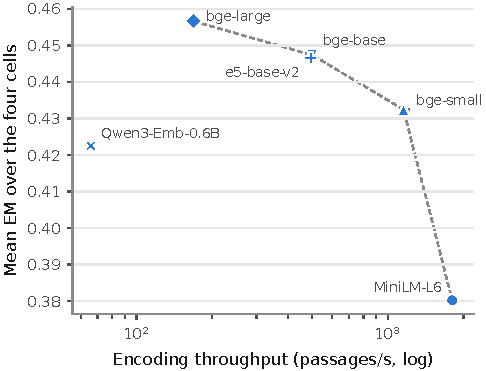
\includegraphics[width=0.6\linewidth]{figs/fig5_cost_quality.pdf}
\caption{Encoding throughput on one T4 GPU (median of five repetitions, log scale) against EM averaged over the four reader--dataset cells. The dashed line joins encoders that no other encoder beats on both axes.}
\label{fig:cost}
\end{figure}

\begin{table}[t]
\centering
\small
\caption{Encoding cost on one Tesla T4, median (range) over five repetitions.}
\label{tab:cost}
\begin{tabular}{lrrcc}
\toprule
Encoder & Params (M) & Dim & Passages/s & Query ms \\
\midrule
MiniLM-L6 & 23 & 384 & 1807 (1768--1863) & 6.0 (6.0--6.1) \\
bge-small & 33 & 384 & 1155 (1136--1207) & 10.3 (10.1--10.3) \\
bge-base & 109 & 768 & 502 (501--503) & 10.0 (9.9--10.1) \\
e5-base-v2 & 109 & 768 & 493 (491--496) & 10.0 (9.9--10.1) \\
bge-large & 335 & 1024 & 168 (168--169) & 18.3 (18.3--18.6) \\
Qwen3-Emb-0.6B & 596 & 1024 & 66 (66--66) & 52.2 (51.8--54.9) \\
\bottomrule
\end{tabular}
\par\smallskip\parbox{\linewidth}{\footnotesize BM25 batch-1 query latency on CPU: 25.7 ms (23.7--27.7).}
\end{table}


\paragraph{Approximate search}
HNSW search kept the exact top five almost unchanged (Table~\ref{tab:hnsw}). At efSearch 128 the top-5 overlap with exact search was \ev{E6.ov5.R2} or higher, Hit@5 changed by at most \ev{E6.dhitabs.max}, and the median query latency on the CPU fell from \ev{E6.lat.exact.R1}--\ev{E6.lat.exact.R5}~ms to \ev{E6.lat.ef128.R1}--\ev{E6.lat.ef128.R5}~ms.

\begin{table*}[t]
\centering
\small
\caption{Approximate search (HNSW, $M{=}32$) vs exact search on the NQ sub-corpus, CPU.}
\label{tab:hnsw}
\begin{tabular}{lcccccccc}
\toprule
Encoder & \multicolumn{2}{c}{Exact} & \multicolumn{3}{c}{HNSW ef=64} & \multicolumn{3}{c}{HNSW ef=128} \\ & Hit@5 & ms & Overlap & Hit@5 & ms & Overlap & Hit@5 & ms \\
\midrule
MiniLM-L6 & 0.673 & 35.9 & 0.946 & 0.672 & 0.50 & 0.984 & 0.673 & 0.84 \\
bge-small & 0.729 & 36.3 & 0.904 & 0.726 & 0.49 & 0.964 & 0.727 & 0.89 \\
e5-base-v2 & 0.817 & 77.7 & 0.915 & 0.815 & 0.80 & 0.970 & 0.817 & 1.45 \\
\bottomrule
\end{tabular}
\par\smallskip\parbox{\linewidth}{\footnotesize Overlap: mean share of the exact top 100 recovered. ms: median batch-1 query latency on 4 vCPUs.}
\end{table*}


\paragraph{Sub-corpus versus full corpus}
On the full NQ corpus the four tested retrievers kept their nDCG@10 order (Kendall's $\tau$ = \ev{E9.tau}; P3 held; Table~\ref{tab:fullcorpus} and Fig.~\ref{fig:fullcorpus}). The dense retrievers lost \ev{E9.dropabs.R2} to \ev{E9.dropabs.R1} in nDCG@10, and BM25 lost almost nothing (\ev{E9.dropabs.R0}). The sub-corpus therefore inflates absolute dense scores but not their order. Its BM25-mined negatives may also make the sub-corpus easier for BM25 relative to the dense encoders than the full corpus is; we did not test reader answers on the full corpus.

\begin{figure}[t]
\centering
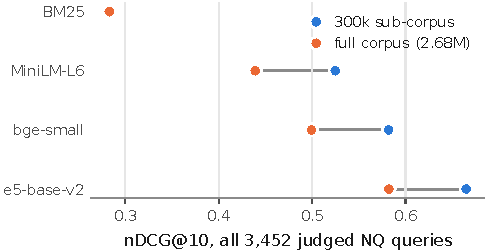
\includegraphics[width=0.6\linewidth]{figs/fig6_full_corpus.pdf}
\caption{nDCG@10 on the 300,000-passage sub-corpus and on the full NQ corpus (all 3,452 judged queries).}
\label{fig:fullcorpus}
\end{figure}

\begin{table}[t]
\centering
\small
\caption{Sub-corpus (300k) vs full NQ corpus (2.68M), all 3,452 judged queries.}
\label{tab:fullcorpus}
\begin{tabular}{lcccc}
\toprule
Retriever & nDCG@10 sub & nDCG@10 full & Hit@5 sub & Hit@5 full \\
\midrule
BM25 & 0.284 & 0.283 & 0.373 & 0.373 \\
MiniLM-L6 & 0.525 & 0.439 & 0.673 & 0.571 \\
bge-small & 0.582 & 0.499 & 0.729 & 0.630 \\
e5-base-v2 & 0.665 & 0.582 & 0.817 & 0.727 \\
\bottomrule
\end{tabular}
\par\smallskip\parbox{\linewidth}{\footnotesize Kendall's $\tau$ between the two orderings = 1.00.}
\end{table}


\subsection{LLM judge validation}\label{sec:res-judge}
The LLM judge agreed poorly with the author's labels (Table~\ref{tab:judge}). Cohen's $\kappa$ was \ev{JA.kappa} \ev{JA.ci}, with raw agreement \ev{JA.raw}. Weighted to the population, the judge labelled \ev{JA.jrate} of answers as supported, against \ev{JA.hrate} for the author, and its precision for the label supported was \ev{JA.prec}. Under the registered rule ($\kappa<0.2$) we excluded the judge's faithfulness labels from all conclusions.

\begin{table}[t]
\centering
\small
\caption{Agreement between the author's labels and the LLM judge on 200 stratified items.}
\label{tab:judge}
\begin{tabular}{lcc}
\toprule
& Judge SUPPORTED & Judge NOT\_SUPPORTED \\
\midrule
Human SUPPORTED & 65 & 50 \\
Human NOT\_SUPPORTED & 37 & 48 \\
\bottomrule
\end{tabular}
\par\smallskip\parbox{\linewidth}{\footnotesize Cohen's $\kappa$ = 0.127 [$-$0.006, 0.261]; raw agreement 0.565. Under the pre-registered rule ($\kappa<0.2$) the judge results are excluded from the conclusions.}
\end{table}


\subsection{Summary of the predictions}
Table~\ref{tab:predictions} lists all six predictions. P3, P4 and P5 held. P1 failed in one of three new cells, P2 failed in both HotpotQA cells, and P6 failed. Where a verdict is not confirmatory, the table marks it.

\begin{table*}[t]
\centering
\small
\caption{Pre-registered predictions and their outcomes.}
\label{tab:predictions}
\begin{tabular}{lllp{0.55\linewidth}}
\toprule
ID & Scope & Result & Evidence \\
\midrule
P1 & NQ, Qwen$^\dagger$ & holds & 6 ratios; largest upper bound 0.455 (Qwen3-Emb-0.6B) \\
P1 & NQ, Llama & holds & 6 ratios; largest upper bound 0.427 (bge-small) \\
P1 & HotpotQA, Qwen & holds & 5 ratios; largest upper bound 0.996 (bge-large) \\
P1 & HotpotQA, Llama & \textbf{fails} & 5 ratios; largest upper bound 1.096 (bge-large) \\
P2 & NQ, Qwen$^\dagger$ & holds & bge-large $-$ e5: $-$0.006 ($p_\text{Holm}$ 1.000); Qwen3-Emb-0.6B $-$ e5: $-$0.018 ($p_\text{Holm}$ 0.271) \\
P2 & NQ, Llama & holds & bge-large $-$ e5: $-$0.004 ($p_\text{Holm}$ 1.000); Qwen3-Emb-0.6B $-$ e5: $-$0.007 ($p_\text{Holm}$ 1.000) \\
P2 & HotpotQA, Qwen & \textbf{fails} & bge-large $-$ e5: +0.028 ($p_\text{Holm}$ 0.005); Qwen3-Emb-0.6B $-$ e5: $-$0.030 ($p_\text{Holm}$ 0.003) \\
P2 & HotpotQA, Llama & \textbf{fails} & bge-large $-$ e5: +0.022 ($p_\text{Holm}$ 0.040); Qwen3-Emb-0.6B $-$ e5: $-$0.042 ($p_\text{Holm}$ $<$0.001) \\
P3 & NQ, 4 retrievers & holds & Kendall's $\tau$ = 1.00 \\
P4 & NQ, Qwen & holds & $k{=}1$ below $k{=}5$ for all 7 retrievers$^\ddagger$; $\Delta$EM $-$0.126 to $-$0.078; all $p_\text{Holm}$ $<$0.001 \\
P5 & NQ, Qwen, 500 q. & holds & hard vs random negatives: $\Delta$EM $-$0.074, $p$ $<$0.001 \\
P6 & NQ, Qwen, 500 q. & \textbf{fails} & gold at position 1/3/5: largest $|\Delta$EM$|$ 0.016; smallest $p_\text{Holm}$ 0.94 \\
\bottomrule
\end{tabular}
\par\smallskip\parbox{\linewidth}{\footnotesize P1: every reportable EM transfer ratio has an upper 95\% bound below 1. P2: no Holm-significant EM gain of bge-large or Qwen3-Emb-0.6B over e5-base-v2. P3: the full corpus keeps the nDCG@10 ordering. P4: EM at $k{=}1$ below $k{=}5$. P5: hard negatives lower EM. P6: gold position changes EM. $^\dagger$Not confirmatory: this cell was observed in Phase 1 of the study, before the predictions were registered. $^\ddagger$Confirmatory for bge-small, bge-base, e5-base-v2 and Qwen3-Emb-0.6B only; the other three were observed before registration.}
\end{table*}

